\documentclass{article}
\usepackage{tikz}
\usetikzlibrary{patterns,shadings}
\begin{document}
% 画笔属性
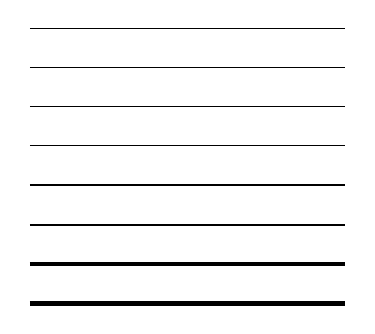
\begin{tikzpicture}
    % 线条粗细: line width, 也可使用以下预定义宽度: ultra thin/very thin/thin(默认)/semithick/thick/very thick/ultra thick
    \draw[ultra thin] (-2,1) -- (2,1);
    \draw[very thin] (-2,0.5) -- (2,0.5);
    \draw[thin] (-2,0) -- (2,0);
    \draw (-2,-0.5) -- (2,-0.5);
    \draw[semithick] (-2,-1) -- (2,-1);
    \draw[thick] (-2,-1.5) -- (2,-1.5);
    \draw[very thick] (-2,-2) -- (2,-2);
    \draw[ultra thick] (-2,-2.5) -- (2,-2.5);
\end{tikzpicture}\\\vspace{1cm}

\begin{tikzpicture}
    % 线条类型: tikz的线条主要由虚线来实现
    % 1.dash pattern=on 2pt off 3pt on 4pt off 4pt
    % 代表画2pt线条,间隔3pt,再画4pt线条,再间隔4pt
    % 2.dash phase=3pt
    % 将通过dash pattern配置的虚线,左移3pt
    % 3.dash=<pattern> phase <phase>
    % 合并1/2步
    % 4.其他预定义线条
    %   1)solid - 实线. 默认类型
    %   2)dotted/densely dotted/loosely dotted - 点线/密集点线/稀疏点线
    %   3)dashed/densely dashed/loosely dashed - 虚线/密集虚线/稀疏虚线
    %   4)dash dot/densely dash dot/loosely dash dot - 虚点线/密集虚点线/稀疏虚点线
    %   5)dash dot dot/densely dash dot dot/loosely dash dot dot - 虚点点线/密集虚点点线/稀疏虚点点线
    \draw[loosely dashed] (-2,0) -- (2,0);
    \draw[dashed] (-2,-0.5) -- (2,-0.5);
    \draw[densely dashed] (-2,-1) -- (2,-1);
    \draw (-2,-1.5) -- (2,-1.5);
    \draw[solid] (-2,-2) -- (2,-2);
    \draw[loosely dotted] (-2,-2.5) -- (2,-2.5);
    \draw[dotted] (-2,-3) -- (2,-3);
    \draw[densely dotted] (-2,-3.5) -- (2,-3.5);
\end{tikzpicture}\\\vspace{1cm}

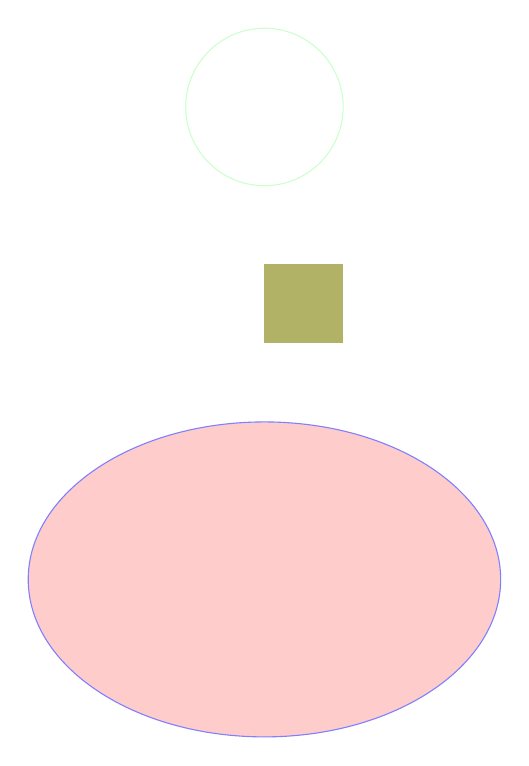
\begin{tikzpicture}
    % 填充颜色: 参考xcolor宏包的颜色表达式
    % draw命令中, color指定边框颜色
    \draw[color=green!20] (0,3) circle [radius=1cm];
    % fill命令中, color指定填充颜色
    \fill[color=red!50!green!60] (0,0) rectangle (1,1);
    % filldraw命令中,color指定填充和边框颜色,fill指定填充颜色,draw指定边框颜色
    \filldraw[color=blue!50,fill=red!20] (0,-3) ellipse [x radius=3cm,y radius=2cm];
\end{tikzpicture}\\\vspace{1cm}

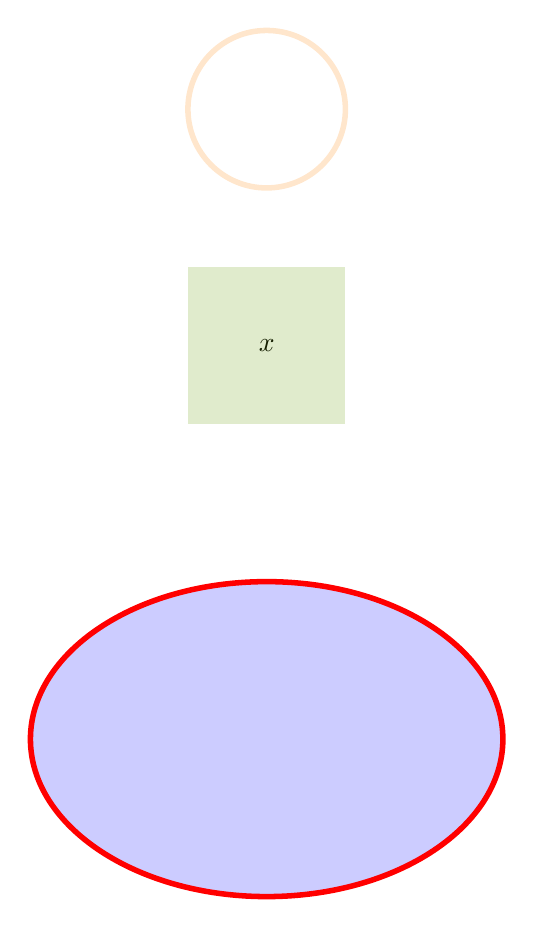
\begin{tikzpicture}
    % 透明度,范围[0,1],0代表完全透明,1代表完全不透明
    \node at (0,0) {$x$};
    % draw中,opacity指定边框透明度
    \draw[color=orange,line width=2pt,opacity=0.2] (0,3) circle [radius=1cm];
    % fill中,opacity指定填充透明度
    \fill[color=red!40!green,opacity=0.2] (-1,-1) rectangle (1,1);
    % filldraw中,fill opacity指定填充透明度,draw opacity指定边框透明度,opacity指定填充和边框透明度
    \filldraw[line width=2pt,draw=red,fill=blue,fill opacity=0.2] (0,-5) ellipse [x radius=3cm,y radius=2cm];
\end{tikzpicture}\\\vspace{1cm}

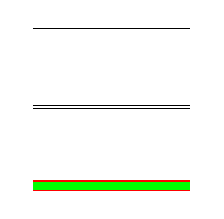
\begin{tikzpicture}
    % 单线与双线
    % 可使用double参数的属性值指定线条间填充颜色
    % double distance指定线条间的距离
    \draw (0,1) -- (2,1);
    \draw[double] (0,0) -- (2,0);
    \draw[double,red,double=green,double distance=3pt] (0,-1) -- (2,-1);
\end{tikzpicture}\\\vspace{1cm}

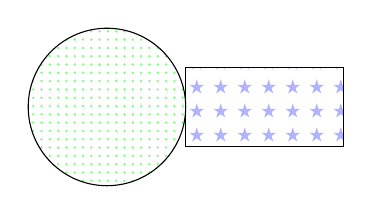
\begin{tikzpicture}
    % 使用预定义图形进行填充, 需要使用patterns库
    % pattern指定填充图形,pattern color指定填充图形的颜色
    \filldraw[pattern=dots,pattern color=green!50] (0,0) circle [radius=1cm];
    \filldraw[pattern=fivepointed stars,pattern color=blue!30] (1,-0.5) rectangle (3,0.5);
\end{tikzpicture}\\\vspace{1cm}

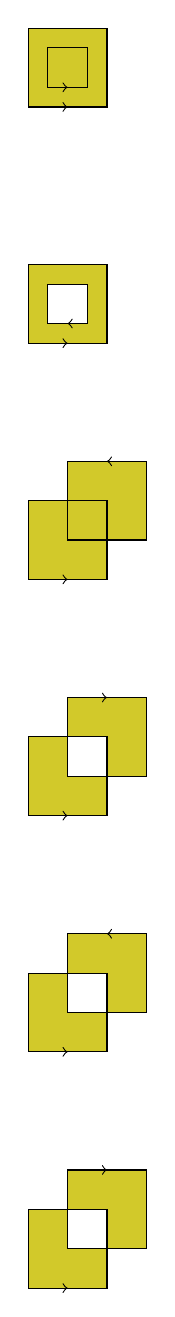
\begin{tikzpicture}
    % 图形重叠部分的填充方式
    % 1.nonzero rule,默认方式,当两个图形同时逆时针/顺时针构成时,重叠部分依然填充;当两个图形分别逆时针和顺时针时,重叠部分留白
    \begin{scope}
	\filldraw[fill=yellow!80!black]
	(0,0) -- (1,0) -- (1,1) -- (0,1) -- cycle
	(0.25,0.25) -- (0.75,0.25) -- (0.75,0.75) -- (0.25,0.75) -- cycle;
	\draw[->] (0,0) -- (0.5,0);
	\draw[->] (0.25,0.25) -- (0.5,0.25);
    \end{scope}
    \begin{scope}[yshift=-3cm]
	\filldraw[fill=yellow!80!black]
	(0,0) -- (1,0) -- (1,1) -- (0,1) -- cycle
	(0.25,0.25) -- (0.25,0.75) -- (0.75,0.75) -- (0.75,0.25) -- cycle;
	\draw[->] (0,0) -- (0.5,0);
	\draw[->] (0.75,0.25) -- (0.5,0.25);
    \end{scope}
    \begin{scope}[yshift=-6cm]
	\filldraw[fill=yellow!80!black]
	(0,0) -- (1,0) -- (1,1) -- (0,1) -- cycle
	(0.5,0.5) -- (1.5,0.5) -- (1.5,1.5) -- (0.5,1.5) -- cycle; 
	\draw[->] (0,0) -- (0.5,0);
	\draw[->] (1.5,1.5) -- (1,1.5);
    \end{scope}
    \begin{scope}[yshift=-9cm]
	\filldraw[fill=yellow!80!black]
	(0,0) -- (1,0) -- (1,1) -- (0,1) -- cycle
	(0.5,0.5) -- (0.5,1.5) -- (1.5,1.5) -- (1.5,0.5) -- cycle; 
	\draw[->] (0,0) -- (0.5,0);
	\draw[->] (0.5,1.5) -- (1,1.5);
    \end{scope}

    % 2.even odd rule,图形相交部分直接留白
    \begin{scope}[yshift=-12cm]
	\filldraw[even odd rule,fill=yellow!80!black]
	(0,0) -- (1,0) -- (1,1) -- (0,1) -- cycle
	(0.5,0.5) -- (1.5,0.5) -- (1.5,1.5) -- (0.5,1.5) -- cycle; 
	\draw[->] (0,0) -- (0.5,0);
	\draw[->] (1.5,1.5) -- (1,1.5);
    \end{scope}
    \begin{scope}[yshift=-15cm]
	\filldraw[even odd rule,fill=yellow!80!black]
	(0,0) -- (1,0) -- (1,1) -- (0,1) -- cycle
	(0.5,0.5) -- (0.5,1.5) -- (1.5,1.5) -- (1.5,0.5) -- cycle; 
	\draw[->] (0,0) -- (0.5,0);
	\draw[->] (0.5,1.5) -- (1,1.5);
    \end{scope}
\end{tikzpicture}\\\vspace{1cm}

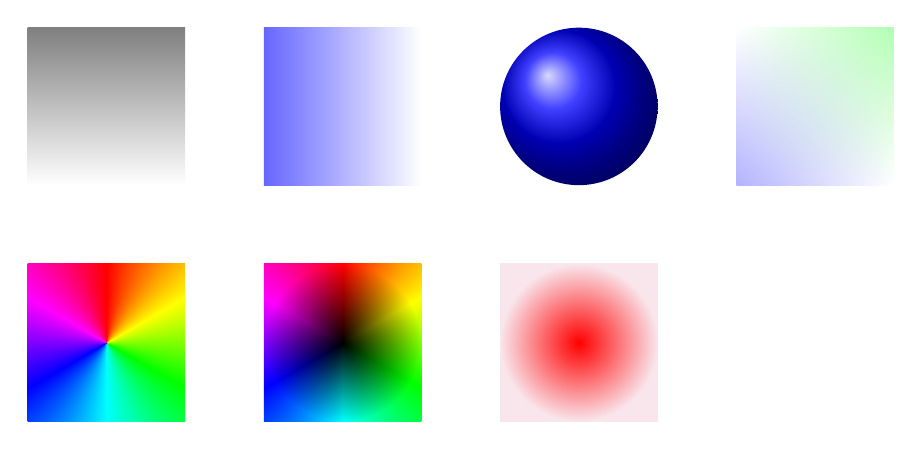
\begin{tikzpicture}
    % shade,填充颜色从一个颜色平滑过渡到另一个颜色,需使用shadings库
    % 1.axis模式, 从左到右或从上到下的线性颜色变化. 默认模式
    % 使用shading=axis指定模式,该模式默认为从上到下,由灰色过渡到白色
    % 可使用如下参数: top color/middle color/bottom color/left color/right color
    \shade (0,0) rectangle (2,2);
    \shade[xshift=3cm,left color=blue!60] (0,0) rectangle (2,2);

    % 2.ball模式, 球体光影变化
    % 使用shading=ball指定模式,默认为蓝色
    % 可使用ball color指定颜色
    \shade[xshift=7cm,shading=ball] (0,1) circle [radius=1cm];

    % 3.bilinear interpolation模式,双线性
    % 使用shading=bilinear interpolation指定模式
    % 可使用以下关键字指定左上/右上/左下/右下颜色: upper left/upper right/lower left/lower right,默认都为白色
    \shade[xshift=9cm,shading=bilinear interpolation,upper right=green!30,lower left=blue!30] (0,0) rectangle (2,2);

    % 4.color wheel模式,车轮式颜色轮替
    % 使用shading=color wheel指定模式
    \shade[yshift=-3cm,shading=color wheel] (0,0) rectangle (2,2);

    % 5.color wheel black center模式,车轮式颜色轮替,中心为黑色
    % 使用shading=color wheel black center指定模式
    \shade[shift={(3cm,-3cm)},shading=color wheel black center] (0,0) rectangle (2,2);

    % 6.radial模式,由一点以半径向外扩散转化颜色
    % 使用shading=radial指定模式
    % 使用inner color指定中心颜色,outer color指定边缘颜色. 默认圆心为灰色,边缘颜色为白色
    \shade[shift={(6cm,-3cm)},shading=radial,inner color=red,outer color=purple!10] (0,0) rectangle (2,2);
\end{tikzpicture}\\\vspace{1cm}

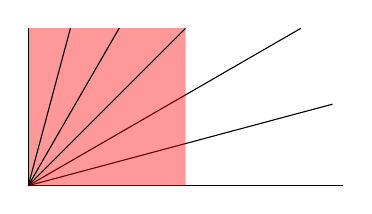
\begin{tikzpicture}
    % clip,针对该指令之后的内容,只保留该指令限定区域部分;指令之前的内容,不作区域限制
    \draw (0,0) -- (0:4cm);
    \draw (0,0) -- (15:4cm);
    \draw (0,0) -- (30:4cm);
    \clip (0,0) rectangle (2,2);
    \fill[red,opacity=0.4] (0,0) rectangle (2,2);
    \draw (0,0) -- (45:4cm);
    \draw (0,0) -- (60:4cm);
    \draw (0,0) -- (75:4cm);
    \draw (0,0) -- (90:4cm);
\end{tikzpicture}\\\vspace{1cm}

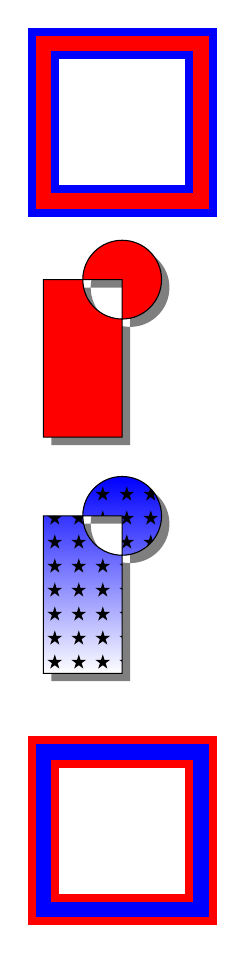
\begin{tikzpicture}
    % preaction(pre-action)参数,先进行preaction的操作,再使用指定参数作图后
    % 如图示例,先作一个宽度为2mm,颜色为蓝色的矩形;再画一个红色的矩形
    \draw 
    [preaction={draw,line width=4mm,blue}]
    [line width=2mm,red] (0,0) rectangle (2,2);
    \begin{scope}[yshift=-3cm]
	\draw 
	[preaction={fill=black,opacity=0.5,transform canvas={xshift=1mm,yshift=-1mm}}]
	[fill=red] (0,0) rectangle (1,2) circle (5mm);
    \end{scope}
    % 多次调用preaction
    \begin{scope}[yshift=-6cm]
	\draw 
	[preaction={fill=black,opacity=0.5,transform canvas={xshift=1mm,yshift=-1mm}}]
	[preaction={top color=blue,bottom color=white}]
	[pattern=fivepointed stars] (0,0) rectangle (1,2) circle (5mm);
    \end{scope}
    \begin{scope}[yshift=-9cm]
	\draw 
	[postaction={draw,line width=2mm,blue}]
	[line width=4mm,red] (0,0) rectangle (2,2);
    \end{scope}
\end{tikzpicture}
\end{document}
